%%%%%%%%%%%%%%%%%%%%%%%%%%%%%%%%%%%%%%%%%%%%%%%%%%%%%%%%%%%%%%%%%%%%%%%%%%%%%%%%%%
\begin{frame}[fragile]\frametitle{}
\begin{center}
{\Large Random Forest}
\end{center}
\end{frame}


%%%%%%%%%%%%%%%%%%%%%%%%%%%%%%%%%%%%%%%%%%%%%%%%%%%%%%%%%%
\begin{frame}[fragile]\frametitle{Random Forests}
\begin{itemize}
\item Leo Breiman managed to apply bootstrapping not only in statistics but also in machine learning. \item He, along with Adel Cutler, extended and improved the random forest algorithm proposed by Tin Kam Ho. 
\item They combined the construction of uncorrelated trees using CART, bagging, and the random subspace method.
\item Decision trees are a good choice for the base classifier in bagging because they are quite sophisticated and can achieve zero classification error on any sample. 

\end{itemize}

See ``Working with Leo Breiman on Random Forests, Adele Cutler'' video at Youtube.
\end{frame}



%%%%%%%%%%%%%%%%%%%%%%%%%%%%%%%%%%%%%%%%%%%%%%%%%%%%%%%%%%
\begin{frame}[fragile]\frametitle{Random Forests}
\begin{itemize}
\item Actually a bagging algorithm
\item Also here, we draw random bootstrap samples from our training set.
\item However, in addition to the bootstrap samples, we also draw random subsets of features for training the individual trees; 
\item In bagging, we provide each tree with the full set of features. 
\item Due to the random feature selection, the trees are more independent of each other compared to regular bagging, which often results in better predictive performance (due to better variance-bias trade-offs), and it's also faster than bagging, because each tree learns only from a subset of features.

\end{itemize}
\end{frame}




%%%%%%%%%%%%%%%%%%%%%%%%%%%%%%%%%%%%%%%%%%%%%%%%%%%%%%%%%%
\begin{frame}[fragile]\frametitle{Random Forest}
\begin{center}
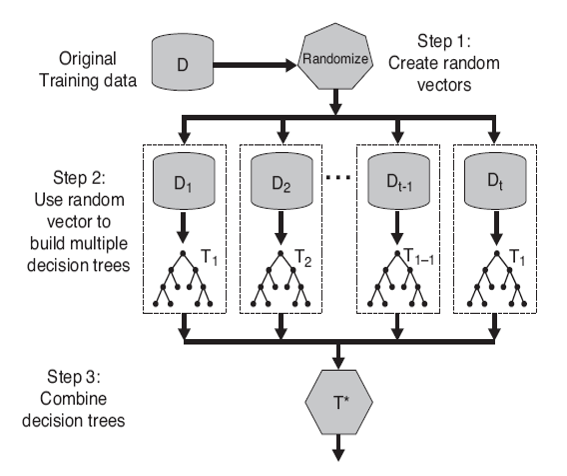
\includegraphics[width=0.8\linewidth,keepaspectratio]{randfor}
\end{center}
\end{frame}







%%%%%%%%%%%%%%%%%%%%%%%%%%%%%%%%%%%%%%%%%%%%%%%%%%%
\begin{frame}[fragile] \frametitle{Random Forests}

\begin{itemize}
\item Random forests fit many decision trees to the same training data.
\item First takes a random sample of features to grow each decision tree.
\item Evaluate. Compare with previous trees.
\item A forest is produced.
\item A joint classification model is produced using all the trees.
\end{itemize}
\end{frame}

%%%%%%%%%%%%%%%%%%%%%%%%%%%%%%%%%%%%%%%%%%%%%%%%%%%%%%%%%%
\begin{frame}[fragile]\frametitle{Random Forest Algorithm}
\begin{itemize}
\item Let the number of instances be equal to $\ell$, and the number of feature dimensions be equal to $d$.
\item Choose $L$ as the number of individual models in the ensemble.
\item For each model $l$, choose the number of features $dl<d$. As a rule, the same value of $dl$ is used for all the models.
\item For each model $l$, create a training set by selecting $dl$ features at random from the whole set of $d$ features.
\item Train each model.
\item Apply the resulting ensemble model to a new instance by combining the results from all the models in $L$. You can use either majority voting or aggregation of the posterior probabilities.

\end{itemize}
\end{frame}


%%%%%%%%%%%%%%%%%%%%%%%%%%%%%%%%%%%%%%%%%%%%%%%%%%%%%%%%%%
\begin{frame}[fragile]\frametitle{Random Forest Algorithm}
Constructing a random forest of $N$ trees goes as follows:
\begin{itemize}
\item For each $k = 1, \dots, N$:
\begin{itemize}
\item  Generate a bootstrap sample $X_k$.
\item  Build a decision tree $b_k$ on the sample $X_k$:
\begin{itemize}
\item Pick the best feature dimension according to the given criteria. 
\item Split the sample by this feature to create a new tree level. Repeat this procedure until the sample is exhausted.
\item Building the tree until any of its leaves contains no more than $n_{min}$ instances or until a certain depth is reached.
\item For each split, we first randomly pick $m$ features from the $d$ original ones and then search for the next best split only among the subset.
\end{itemize}
\end{itemize}
\end{itemize}
\end{frame}


%%%%%%%%%%%%%%%%%%%%%%%%%%%%%%%%%%%%%%%%%%%%%%%%%%%%%%%%%%
\begin{frame}[fragile]\frametitle{Random Forest Algorithm}
The final classifier is defined by:

$a(x) = \frac{1}{N}\sum_{k = 1}^N b_k(x)$

\begin{itemize}
\item We use the majority voting for classification and the mean for regression.
\item For classification problems, it is advisable to set $m = \sqrt{d}$. 
\item For regression problems, we usually take $m = \frac{d}{3}$, where $d$ is the number of features. \item It is recommended to build each tree until all of its leaves contain only $ n_\text{min} = 1$ examples for classification and $n_\text{min} = 5$ examples for regression.
\item You can see random forest as bagging of decision trees with the modification of selecting a random subset of features at each split.
\end{itemize}

\end{frame}


%%%%%%%%%%%%%%%%%%%%%%%%%%%%%%%%%%%%%%%%%%%%%%%%%%%%%%%%%%
\begin{frame}[fragile]\frametitle{Task}
There are 7 jurors in the courtroom. Each of them individually can correctly determine whether the defendant is guilty or not with 80\% probability. How likely is the jury will make a correct verdict jointly if the decision is made by majority voting?

\begin{itemize}
\item 20.97\%
\item 80.00\%
\item 83.70\%
\item 96.66\%
\end{itemize}
Answer XXX
\end{frame}

%%%%%%%%%%%%%%%%%%%%%%%%%%%%%%%%%%%%%%%%%%%%%%%%%%%%%%%%%%
\begin{frame}[fragile]\frametitle{Random Forest Splits}
\begin{itemize}
\item Selection of random subset of features to determine each split
\item How large should subset be?
\begin{itemize}
\item Typically root(K), for K features works well for classification
\item (K / 3) for regression
\end{itemize}
\item Tree is grown to full size with pruning
\item Overall prediction is majority vote from all individually trained trees
\item Different variations of Random Forests exist
\end{itemize}
\end{frame}



% %%%%%%%%%%%%%%%%%%%%%%%%%%%%%%%%%%%%%%%%%%%%%%%%%%%
% \begin{frame}[fragile] \frametitle{Random Forests}


% \begin{itemize}
% \item Training set for a given tree is sampled from the original
% data, with or without replacement
% \item At each training split, only a randomly chosen subset (of size $m$)
% of the variable are considered for splitting the data
% \end{itemize}
% \end{frame}

% %%%%%%%%%%%%%%%%%%%%%%%%%%%%%%%%%%%%%%%%%%%%%%%%%%%
% \begin{frame}[fragile] \frametitle{Random Forests}

% \begin{itemize}
% \item In order to predict new values from this ensemble of trees, we take the
% predictions from each model
% \item Average them together (for classification,
% the class labels can also be used as `votes').
% \end{itemize}

% \end{frame}



%%%%%%%%%%%%%%%%%%%%%%%%%%%%%%%%%%%%%%%%%%%%%%%%%%%%%%%%%%
\begin{frame}[fragile]\frametitle{Comparison with Decision Trees and Bagging}
\begin{itemize}
\item In a random forest, the best feature for a split is selected from a random subset of the available features while, in bagging, all features are considered for the next best split.
\item ``Normal'' decision tree induction utilizes full set of features to determine each split
\item Random forest injects randomness
\end{itemize}
\end{frame}



%%%%%%%%%%%%%%%%%%%%%%%%%%%%%%%%%%%%%%%%%%%%%%%%%%%%%%%%%%
\begin{frame}[fragile]\frametitle{Pros and cons of random forests}
Pros
\begin{itemize}
\item High prediction accuracy; will perform better than linear algorithms in most problems; the accuracy is comparable with that of boosting.
\item Robust to outliers, thanks to random sampling.
\item Insensitive to the scaling of features as well as any other monotonic transformations due to the random subspace selection.
\item Doesn't require fine-grained parameter tuning, works quite well out-of-the-box. With tuning, it is possible to achieve a 0.5–3% gain in accuracy, depending on the problem setting and data.
\item Efficient for datasets with a large number of features and classes.
\item Handles both continuous and discrete variables equally well.
\end{itemize}
\end{frame}

%%%%%%%%%%%%%%%%%%%%%%%%%%%%%%%%%%%%%%%%%%%%%%%%%%%%%%%%%%
\begin{frame}[fragile]\frametitle{Pros and cons of random forests}
Pros
\begin{itemize}
\item Rarely overfits. In practice, an increase in the tree number almost always improves the composition. But, after reaching a certain number of trees, the learning curve is very close to the asymptote.
\item There are developed methods to estimate feature importance.
\item Works well with missing data
\item Provides means to weight classes on the whole dataset as well as for each tree sample.
\item Easily parallelized and highly scalable.
\end{itemize}
\end{frame}


%%%%%%%%%%%%%%%%%%%%%%%%%%%%%%%%%%%%%%%%%%%%%%%%%%%%%%%%%%
\begin{frame}[fragile]\frametitle{Pros and cons of random forests}
Cons
\begin{itemize}
\item In comparison with a single decision tree, Random Forest's output is more difficult to interpret.
\item There are no formal p-values for feature significance estimation.
Performs worse than linear methods in the case of sparse data: text inputs, bag of words, etc.
\item Unlike linear regression, Random Forest is unable to extrapolate. But, this can be also regarded as an advantage because outliers do not cause extreme values in Random Forests.
\item In the case of categorical variables with varying level numbers, random forests favor variables with a greater number of levels. The tree will fit more towards a feature with many levels because this gains greater accuracy.
\item The resulting model is large and requires a lot of RAM.
\end{itemize}
\end{frame}



%%%%%%%%%%%%%%%%%%%%%%%%%%%%%%%%%%%%%%%%%%%%%%%%%%%%%%%%%%%%%%%%%%%%%%%%
\begin{frame}[fragile]\frametitle{Random Forest (Recap)}
\begin{itemize}
\item Random Forest is an ensemble technique used for classification, regression.
\item It combines the output of weaker techniques in order to get a stronger result.
\item The weaker technique in this case is a decision tree. 
\end{itemize}
\end{frame}

%%%%%%%%%%%%%%%%%%%%%%%%%%%%%%%%%%%%%%%%%%%%%%%%%%%%%%%%%%%%%%%%%%%%%%%%
\begin{frame}[fragile]\frametitle{Random Forest (Recap)}
\begin{itemize}
\item Decision trees work by splitting the and re-splitting the data by features. 
\item If a decision tree is split along good features, it can give a decent predictive output.
\item Random Forest works by averaging decision tree output, but it's a bit more complicated than that.
\end{itemize}
\end{frame}

%%%%%%%%%%%%%%%%%%%%%%%%%%%%%%%%%%%%%%%%%%%%%%%%%%%%%%%%%%%%%%%%%%%%%%%%
\begin{frame}[fragile]\frametitle{Random Forest (Recap)}
\begin{itemize}
\item It also ranks an individual tree's output, by comparing it to the known output from the training data. 
\item This allows it to rank features. Some of the decision trees will perform better, and so the features within the tree will be deemed more important.
\end{itemize}
\end{frame}





